\documentclass[11pt,a4paper,oneside]{report}
\newcommand{\ReportShortTitle}{Pricing and Hedging European Options}
% Shared layout: title page, executive summary, centred red chapter titles,
% blue small-caps sections, running header. Compile with pdflatex.
\usepackage[T1]{fontenc}
\usepackage[utf8]{inputenc}
\usepackage{charter}
\usepackage[scaled=0.92]{helvet}
\usepackage{amsmath,amssymb}
\usepackage[a4paper,margin=2.3cm,headheight=28pt]{geometry}
\usepackage{graphicx,booktabs,xcolor,titlesec,fancyhdr,enumitem,listings,float,caption}
\usepackage[hidelinks]{hyperref}
\definecolor{navy}{HTML}{0B3A5B}
\definecolor{accent}{HTML}{D6312B}
\definecolor{secblue}{HTML}{1E6A8D}
\definecolor{codebg}{HTML}{F3F1EA}
\setlength{\parindent}{1.5em}
\setlength{\parskip}{3pt}
\linespread{1.05}
\newcommand{\ornament}{\par\vspace{2pt}{\centering\color{accent}\rule{2.2cm}{0.4pt}\hspace{2pt}\rule[-1pt]{1.2cm}{2.2pt}\hspace{2pt}\rule{2.2cm}{0.4pt}\par}\vspace{6pt}}
\titleformat{\chapter}[display]{\centering\sffamily\bfseries\color{accent}}{\Large\thechapter}{2pt}{\LARGE\MakeUppercase}[\ornament]
\titlespacing*{\chapter}{0pt}{-10pt}{14pt}
\titleformat{name=\chapter,numberless}[display]{\centering\sffamily\bfseries\color{accent}}{}{0pt}{\LARGE\MakeUppercase}[\ornament]
\titlespacing*{name=\chapter,numberless}{0pt}{-10pt}{14pt}
\titleformat{\section}{\Large\scshape\color{secblue}}{\thesection}{0.6em}{}[{\color{secblue}\vspace{-4pt}\rule{1.1cm}{2pt}}]
\titleformat{\subsection}{\large\scshape\color{secblue}}{\thesubsection\enspace$\bullet$}{0.5em}{}
\pagestyle{fancy}
\fancyhf{}
\fancyhead[L]{\color{navy}\scshape\small\ReportShortTitle}
\fancyfoot[C]{\color{navy}\rule[3pt]{0.5cm}{0.4pt}\\\thepage}
\renewcommand{\headrulewidth}{0pt}
\fancypagestyle{plain}{\fancyhf{}\fancyhead[L]{\color{navy}\scshape\small\ReportShortTitle}\fancyfoot[C]{\color{navy}\rule[3pt]{0.5cm}{0.4pt}\\\thepage}\renewcommand{\headrulewidth}{0pt}}
\captionsetup{font=small,labelfont=sc}
\lstset{basicstyle=\ttfamily\footnotesize,backgroundcolor=\color{codebg},frame=none,
  keywordstyle=\color{accent},commentstyle=\color{gray},numbers=left,
  numberstyle=\tiny\color{gray},language=Python,breaklines=true,columns=fullflexible,xleftmargin=1.5em}
\newcommand{\maketitlepage}[5]{% title, subtitle, date, author, repo
\begin{titlepage}\centering
\vspace*{5cm}
{\sffamily\bfseries\color{navy}\fontsize{26}{32}\selectfont\MakeUppercase{#1}\par}
\vspace{2.2cm}
{\sffamily\bfseries\color{navy}\Large #2\par}
\vspace{4.5cm}
{\color{navy}\large #3\par}
\vspace{4pt}{\color{navy}\rule{1.2cm}{2pt}\par}\vspace{8pt}
{\color{navy}\large #4\par}
\vspace{6pt}{\color{navy}\small\texttt{#5}\par}
\vfill
{\color{navy}\small Independent research project\par}
\end{titlepage}}


\begin{document}
\maketitlepage{Pricing and Hedging European Options}
{Three Numerical Methods, Their Cost, and What Discrete Hedging Really Leaves Behind}
{October 2026}{Stéphane N'Da}{github.com/StephaneMian/bs-pricing-hedging}

\chapter*{Executive Summary}
\thispagestyle{plain}

The Black--Scholes model gives a closed-form price for a European option, which makes it an ideal test bench: every numerical method can be checked against an exact answer, and every error can be measured rather than guessed. This project uses that property to answer two practical questions.

The first is a question of numerical method. The same call option is priced by Monte Carlo simulation (plain, antithetic variates, control variate), by a finite-difference solution of the pricing PDE, and in closed form. For a one-dimensional problem the PDE is far more efficient: a Crank--Nicolson grid reaches an error of $4\times10^{-5}$ in about 70\,ms, whereas two million Monte Carlo paths leave an error of about $10^{-2}$ in comparable time. The measured order of convergence of the PDE scheme is $2.00$. Variance reduction matters, but its value depends on the contract: the control variate divides the variance by 50 for a deep in-the-money call and only by 2 for an out-of-the-money one. A second finding concerns Greeks rather than prices. Plain Crank--Nicolson produces a price that is correct to second order but a gamma that oscillates near the strike, with a maximum error of 10.7 against a true value of 0.06. Two implicit start-up steps (Rannacher smoothing) bring that error down to $2\times10^{-4}$.

The second question is what a trader keeps when hedging in discrete time. A short call hedged $N$ times over one year leaves a P\&L whose standard deviation decreases as $N^{-0.489}$ in simulation, close to the theoretical $N^{-1/2}$ and within 8\% of the Derman--Kamal approximation at every frequency tested. When the option is sold at 20\% implied volatility but the market realises 25\%, the average loss equals the price difference ($-1.93$ for a premium of 9.41) whichever volatility is used for the hedge ratio. What changes is the dispersion: hedging with the realised volatility halves the standard deviation of the P\&L (0.53 against 0.98), and the remaining dispersion is almost exactly the discretisation error.

All results are reproducible from a single script with fixed seeds, and the pricing functions are covered by unit tests that compare every numerical method with its closed form.

\tableofcontents

%--------------------------------------------------------------------------
\chapter{Setting and Methods}

\section{Model}
Under the risk-neutral measure the stock follows a geometric Brownian motion
\begin{equation}
dS_t = r S_t\,dt + \sigma S_t\,dW_t ,
\end{equation}
with constant rate $r$ and volatility $\sigma$. The price of a European call with strike $K$ and maturity $T$ is
\begin{equation}
C = S_0\,\Phi(d_1) - K e^{-rT}\Phi(d_2),\qquad d_{1,2} = \frac{\ln(S_0/K) + (r\pm\tfrac12\sigma^2)T}{\sigma\sqrt T}.
\end{equation}
Unless stated otherwise the experiments use $S_0=100$, $T=1$, $r=3\%$, $\sigma=20\%$. The at-the-money call is then worth $9.4134$.

\section{Monte Carlo estimators}
The terminal price is simulated exactly, $S_T = S_0\exp\big((r-\tfrac12\sigma^2)T + \sigma\sqrt T Z\big)$ with $Z\sim\mathcal N(0,1)$, so the only error is statistical. Three estimators are compared.

\begin{itemize}[leftmargin=1.5em]
\item \textbf{Plain.} The sample mean of $e^{-rT}(S_T-K)^+$.
\item \textbf{Antithetic variates.} Each draw $Z$ is paired with $-Z$ and the two payoffs are averaged. The standard error is computed on the pair averages, which are independent; computing it on the $2m$ individual payoffs would understate it.
\item \textbf{Control variate.} The discounted terminal price $Y=e^{-rT}S_T$ has known mean $S_0$. The estimator $X-\beta(Y-S_0)$ uses the sample-optimal $\beta=\mathrm{Cov}(X,Y)/\mathrm{Var}(Y)$. Estimating $\beta$ on the same sample introduces a bias of order $1/n$, negligible here.
\end{itemize}

The efficiency of an estimator is measured by its variance per payoff evaluation, so that an antithetic pair counts as two evaluations.

\section{Finite differences}
With $x=\ln S$ and $\tau=T-t$, the price $u(x,\tau)$ solves
\begin{equation}
\partial_\tau u = \tfrac12\sigma^2\,\partial_{xx}u + \big(r-\tfrac12\sigma^2\big)\partial_x u - r u ,
\end{equation}
a constant-coefficient equation, which is why the log transform is used. The grid is centred on $\ln S_0$ and spans $\pm5\sigma\sqrt T$; Dirichlet conditions use the asymptotic prices ($0$ and $S-Ke^{-r\tau}$ for a call). Time stepping is Crank--Nicolson, second order in time and space, with a tridiagonal system solved at each step.

Crank--Nicolson is unconditionally stable but not strongly damping: high-frequency components of the initial condition are multiplied by a factor close to $-1$ at each step when $\Delta\tau/\Delta x^2$ is large. The kink of the payoff at the strike contains exactly such components. The Rannacher variant replaces the first two time steps by four fully implicit half-steps, which damp them before the Crank--Nicolson steps begin.

\section{Monte Carlo Greeks}
Delta is estimated in three ways: the pathwise derivative $e^{-rT}\mathbf 1_{S_T>K}S_T/S_0$, which is valid because the call payoff is Lipschitz; the likelihood-ratio estimator $e^{-rT}(S_T-K)^+ Z/(S_0\sigma\sqrt T)$, which differentiates the density instead of the payoff; and a central bump-and-revalue with common random numbers and a 1\% bump.

\section{Discrete delta hedging}
The seller of one call receives the premium computed with an implied volatility $\sigma_{\text{imp}}$, buys $\Delta$ shares computed with a hedging volatility $\sigma_h$, and rebalances at $N$ equally spaced dates. The stock is simulated under the real-world measure with drift $\mu=8\%$ and volatility $\sigma_{\text{real}}$. Cash earns $r$. The quantity studied is the discounted P\&L at maturity, after paying the option payoff.

For small time steps, Derman and Kamal give the approximation
\begin{equation}\label{eq:dk}
\mathrm{sd}(\text{P\&L}) \approx \sqrt{\frac{\pi}{4}}\;\frac{\sigma\,\mathcal V}{\sqrt N},
\end{equation}
where $\mathcal V$ is the option vega. The $N^{-1/2}$ rate is the testable part of this statement.

%--------------------------------------------------------------------------
\chapter{Results}

\section{Variance reduction depends on the contract}
Table~\ref{tab:vr} reports, for one million payoff evaluations, the price, its standard error, the distance to the closed form in standard errors ($z$), and the variance ratio relative to plain Monte Carlo.

\begin{table}[H]\centering\small
\begin{tabular}{llrrrr}
\toprule
Strike & Estimator & Price & Std.\ error & $z$ & Variance ratio\\
\midrule
80 (ITM) & plain & 23.2063 & 0.0189 & $-0.93$ & 1.0\\
 & antithetic & 23.2329 & 0.0069 & $1.29$ & 7.6\\
 & control variate & 23.2305 & 0.0027 & $2.41$ & 49.5\\
\multicolumn{2}{l}{\quad closed form 23.2240} &&&&\\
100 (ATM) & plain & 9.4018 & 0.0141 & $-0.82$ & 1.0\\
 & antithetic & 9.4281 & 0.0105 & $1.40$ & 1.8\\
 & control variate & 9.4183 & 0.0058 & $0.85$ & 5.9\\
\multicolumn{2}{l}{\quad closed form 9.4134} &&&&\\
120 (OTM) & plain & 2.7577 & 0.0080 & $-1.11$ & 1.0\\
 & antithetic & 2.7765 & 0.0075 & $1.32$ & 1.1\\
 & control variate & 2.7651 & 0.0055 & $-0.26$ & 2.1\\
\multicolumn{2}{l}{\quad closed form 2.7666} &&&&\\
\bottomrule
\end{tabular}
\caption{Monte Carlo estimators with $10^6$ payoff evaluations each.}\label{tab:vr}
\end{table}

The pattern has a simple explanation. Both techniques exploit the correlation between the payoff and the underlying. Deep in the money, the call behaves almost like the forward $S_T-K$, which is linear in $S_T$: the control variate removes nearly all of its variance, and the antithetic pair cancels the linear part of the noise. Out of the money, most paths pay zero and the payoff is a strongly non-linear function of $Z$; correlation with $S_T$ is weak and both gains shrink. A variance ratio measured on one strike should therefore not be quoted as a property of the method.

The $z$-scores lie between $-1.1$ and $2.4$. The value $2.41$ is the largest of nine, which is unremarkable for nine roughly normal draws, and the unit tests use a separate seed and a four-standard-error tolerance.

\section{Accuracy against cost}
Figure~\ref{fig:cost} plots the absolute error against CPU time. For Monte Carlo the error is the root-mean-square error over 30 independent seeds at each sample size.

\begin{figure}[H]\centering
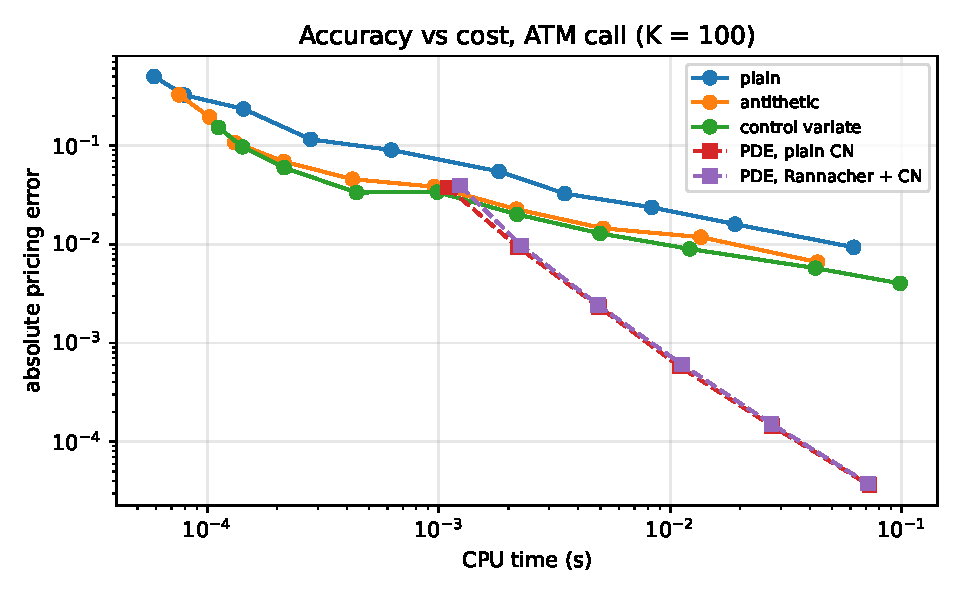
\includegraphics[width=0.8\textwidth]{figures/accuracy_vs_cost.pdf}
\caption{Error against CPU time for the at-the-money call.}\label{fig:cost}
\end{figure}

The Monte Carlo curves have slope close to $-1/2$ in log--log scale, as expected from the central limit theorem, and variance reduction shifts them down without changing the slope. The PDE curve has a slope of about $-1$ in time: halving $\Delta\tau$ and $\Delta x$ quadruples the work and divides the error by four. The fitted order of convergence in the number of time steps is $2.00$. At 800 time steps and 1\,600 space nodes the error is $3.6\times10^{-5}$ in 69\,ms, about 250 times smaller than plain Monte Carlo and 100 times smaller than the control variate at a similar cost.

This ranking is specific to one dimension. The cost of a grid grows exponentially with the number of state variables, while Monte Carlo does not care; for a basket of five assets or a path-dependent payoff the conclusion reverses.

\section{Why Rannacher smoothing matters for Greeks}
For the price at $S_0$, plain Crank--Nicolson and the Rannacher variant give practically the same error at every grid size tested ($3.6\times10^{-5}$ against $3.8\times10^{-5}$ at the finest grid). The difference appears in the gamma, computed from the grid as $(\partial_{xx}u-\partial_x u)/S^2$. Figure~\ref{fig:gamma} uses a short maturity ($T=0.1$) and only ten time steps on a fine space grid, a combination that makes $\Delta\tau/\Delta x^2$ large.

\begin{figure}[H]\centering
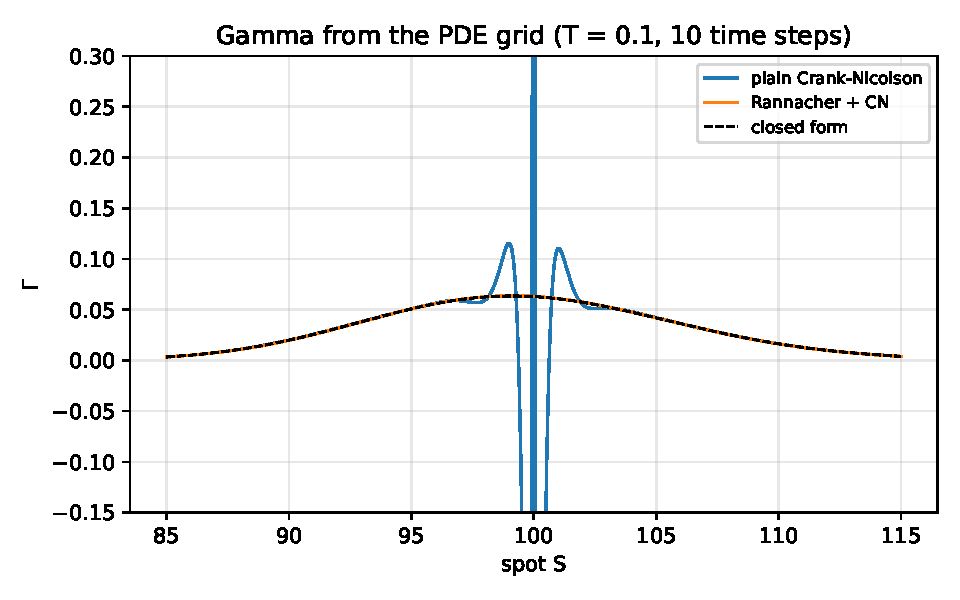
\includegraphics[width=0.75\textwidth]{figures/pde_gamma.pdf}
\caption{Gamma from the PDE grid. The plain scheme spikes to about 10 at the strike; the axis is clipped.}\label{fig:gamma}
\end{figure}

Near the strike the maximum error on gamma is $10.7$ with plain Crank--Nicolson and $1.6\times10^{-4}$ with Rannacher start-up, for a true gamma of about $0.06$. A pricing error of $10^{-4}$ can hide a Greek that is wrong by two orders of magnitude, and a hedger uses the Greek. Testing only the price would not have revealed the problem.

\section{Monte Carlo deltas}
Table~\ref{tab:delta} gives the standard error of each delta estimator with $5\times10^5$ paths.

\begin{table}[H]\centering\small
\begin{tabular}{lrrrr}
\toprule
Strike & True delta & Pathwise & Likelihood ratio & Bump (CRN)\\
\midrule
80 & 0.9140 & $5.4\times10^{-4}$ & $2.8\times10^{-3}$ & $5.3\times10^{-4}$\\
100 & 0.5987 & $8.3\times10^{-4}$ & $2.0\times10^{-3}$ & $8.2\times10^{-4}$\\
120 & 0.2541 & $7.3\times10^{-4}$ & $1.3\times10^{-3}$ & $7.3\times10^{-4}$\\
\bottomrule
\end{tabular}
\caption{Standard errors of three delta estimators ($5\times10^5$ paths).}\label{tab:delta}
\end{table}

The pathwise estimator has between 3 and 27 times less variance than the likelihood ratio. The likelihood ratio multiplies the payoff by $Z$, which adds noise, most visibly in the money where the payoff is large. Its advantage is elsewhere: it does not require a differentiable payoff and remains usable for a digital option, where the pathwise derivative is zero almost everywhere. Bump-and-revalue with common random numbers matches the pathwise estimator, since for a small bump it computes nearly the same quantity, but it needs two full pricings per Greek.

The three estimators were run with the same seed, so their deviations from the true value are correlated: at each strike, all three land about two standard errors below the true delta. This is one draw of the random numbers and not a bias; the unit tests use an independent seed.

\section{Hedging error and rebalancing frequency}
Figure~\ref{fig:freq} shows the standard deviation of the hedging P\&L over 50\,000 paths when all three volatilities equal 20\%.

\begin{figure}[H]\centering
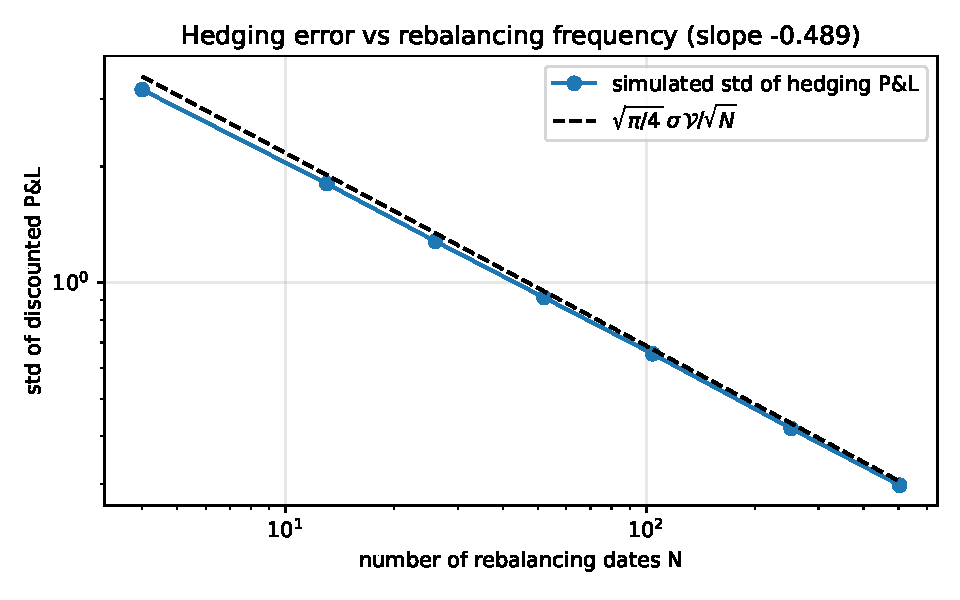
\includegraphics[width=0.75\textwidth]{figures/hedging_frequency.pdf}
\caption{Standard deviation of the discounted P\&L of a delta-hedged short call.}\label{fig:freq}
\end{figure}

\begin{table}[H]\centering\small
\begin{tabular}{lrrrrrrr}
\toprule
$N$ & 4 & 13 & 26 & 52 & 104 & 252 & 504\\
\midrule
Simulated sd & 3.17 & 1.81 & 1.28 & 0.92 & 0.65 & 0.42 & 0.30\\
Approximation \eqref{eq:dk} & 3.43 & 1.90 & 1.34 & 0.95 & 0.67 & 0.43 & 0.31\\
Mean P\&L & $-0.06$ & $-0.01$ & $0.00$ & $0.00$ & $0.00$ & $0.00$ & $0.00$\\
\bottomrule
\end{tabular}
\caption{Hedging P\&L against the number of rebalancing dates, for a premium of 9.41.}
\end{table}

The fitted log--log slope is $-0.489$. The approximation overestimates the dispersion by about 8\% at $N=4$ and by 3\% or less from $N=26$ onwards, which is consistent with its derivation for small steps. The mean P\&L is zero within noise: with correct volatility, discrete hedging adds risk but no expected cost. In practice transaction costs grow linearly with $N$ while the risk falls only as $N^{-1/2}$, which is why desks do not rebalance continuously.

\section{Selling volatility too cheaply}
The option is now sold at $\sigma_{\text{imp}}=20\%$ while the stock realises $\sigma_{\text{real}}=25\%$, with daily rebalancing. Two hedges are compared: delta computed with the implied volatility, and delta computed with the realised one.

\begin{figure}[H]\centering
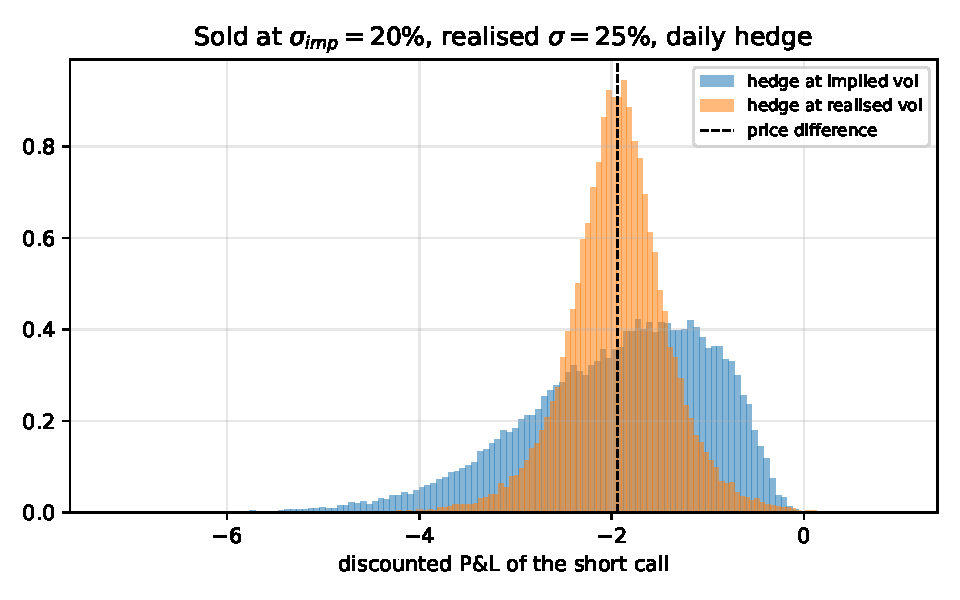
\includegraphics[width=0.75\textwidth]{figures/vol_misspecification.pdf}
\caption{Distribution of the P\&L of a call sold 5 volatility points too cheap.}\label{fig:mis}
\end{figure}

\begin{table}[H]\centering\small
\begin{tabular}{lrrrr}
\toprule
Hedge ratio computed with & Mean & Std & 5\% quantile & 95\% quantile\\
\midrule
implied vol (20\%) & $-1.928$ & 0.975 & $-3.71$ & $-0.60$\\
realised vol (25\%) & $-1.936$ & 0.531 & $-2.81$ & $-1.08$\\
\midrule
$C(\sigma_{\text{imp}})-C(\sigma_{\text{real}})$ & $-1.935$ &&&\\
\bottomrule
\end{tabular}
\caption{Hedging P\&L under volatility misspecification (50\,000 paths).}
\end{table}

Both hedges lose the same amount on average, and that amount is the price difference $C(20\%)-C(25\%)=-1.935$. The choice of hedge volatility changes the shape of the loss, not its expectation.

With the realised volatility the hedge replicates the option that should have been sold, so the loss is locked in at inception and the only remaining noise is the discretisation error. Equation~\eqref{eq:dk} evaluated at 25\% predicts a standard deviation of 0.54 for daily rebalancing; the simulation gives 0.53. With the implied volatility the loss accumulates as $\tfrac12\int\Gamma_t S_t^2(\sigma_{\text{imp}}^2-\sigma_{\text{real}}^2)\,dt$, which depends on the path: it is large when the stock stays near the strike, where gamma is high, and small when it moves away. That path dependence doubles the dispersion.

The practical reading is that a volatility trader does not need to know the future realised volatility to be right on average, but needs it to control the variance of the outcome. Of course the realised volatility is not known in advance; the second hedge is an idealised benchmark.

%--------------------------------------------------------------------------
\chapter{Limits and Extensions}

The Black--Scholes model is used here because it can be solved exactly, not because it describes markets. Three limits bound the conclusions.

\begin{itemize}[leftmargin=1.5em]
\item \textbf{Constant volatility.} The hedging study assumes that the stock follows a GBM with known realised volatility. Real returns have stochastic volatility and jumps, both of which add a component of hedging error that does not vanish as $N$ grows.
\item \textbf{No transaction costs.} The frequency study shows the risk side of the trade-off only. Adding proportional costs would produce an optimal rebalancing frequency, as in Leland's model.
\item \textbf{One dimension.} The advantage of the PDE is specific to a single state variable.
\end{itemize}

The natural next steps are to calibrate a Heston model to an implied volatility surface and repeat the hedging experiment when the hedger uses Black--Scholes deltas in a Heston world, and to add transaction costs in order to recover an optimal rebalancing rule.

\chapter*{References}
\addcontentsline{toc}{chapter}{References}
\begin{enumerate}[label={[\arabic*]},leftmargin=2em]
\item F. Black and M. Scholes, \emph{The Pricing of Options and Corporate Liabilities}, J. Political Economy 81 (1973).
\item P. Glasserman, \emph{Monte Carlo Methods in Financial Engineering}, Springer (2003).
\item R. Rannacher, \emph{Finite element solution of diffusion problems with irregular data}, Numer. Math. 43 (1984).
\item D. J. Duffy, \emph{Finite Difference Methods in Financial Engineering}, Wiley (2006).
\item E. Derman and M. Kamal, \emph{When You Cannot Hedge Continuously: The Corrections of Black--Scholes}, Risk 12 (1999).
\item H. E. Leland, \emph{Option Pricing and Replication with Transactions Costs}, J. Finance 40 (1985).
\end{enumerate}

\chapter*{Appendix: Key Functions}
\addcontentsline{toc}{chapter}{Appendix: Key Functions}
The full code, the tests and the experiment script are in the repository. The functions below are the core of the method.

\section*{Control-variate estimator}
\lstinputlisting[linerange={46-55},firstnumber=46]{../src/bsph/montecarlo.py}

\section*{Discrete delta hedge}
\lstinputlisting[linerange={12-27},firstnumber=12]{../src/bsph/hedging.py}

\end{document}
